% !TEX program = xelatex
\documentclass[a4paper]{article}
\usepackage{amsmath}
\usepackage{amsthm}
\usepackage[left=1.8cm,right=1.8cm,top=2.2cm,bottom=2.0cm]{geometry}
\usepackage{ctex}
\usepackage{enumerate}
\usepackage{fancyhdr}
\usepackage{xpatch}
\usepackage{graphicx} 
\usepackage{float} 
\usepackage{subfigure} 
\usepackage{amsfonts}
\usepackage{mathtools}
\usepackage{framed}
\usepackage{multicol}
\usepackage{listings}
\usepackage{hyperref}
\usepackage{tikz}
\usetikzlibrary{automata,positioning}
\theoremstyle{definition}
\newtheorem*{solution*}{\textbf{Solution:}}
\newtheorem*{proof*}{\textbf{Proof:}}
\newtheorem{theorem}{Theorem}[subsection]
\newtheorem{definition}{Definition}[subsection]
\newtheorem{lemma}{Lemma}[subsection]
\makeatletter
\usepackage{listings}% http://ctan.org/pkg/listings
\lstset{
  basicstyle=\ttfamily\small,
  mathescape,
} 
\AtBeginDocument{\xpatchcmd{\@thm}{\thm@headpunct{.}}{\thm@headpunct{}}{}{}}
\makeatother

\pagestyle{fancy}
\renewcommand{\baselinestretch}{1.15}

\usepackage{paralist}
\let\itemize\compactitem
\let\enditemize\endcompactitem
\let\enumerate\compactenum
\let\endenumerate\endcompactenum
\let\description\compactdesc
\let\enddescription\endcompactdesc

% shorten footnote rule
\xpatchcmd\footnoterule
  {.4\columnwidth}
  {1in}
  {}{\fail}

\title{CS 131 Compilers: Discussion 13: Garbage Collection}
\author{\textbf{杨易为}~~\textbf{季杨彪}~~\textbf{尤存翰} \\ \texttt{ \{yangyw,jiyb,youch\}@shanghaitech.edu.cn}}


\begin{document}
\maketitle
\section{C++ garbage collection}
C++ actually have runtime garbage collection, once put in 2008 and deprecated in 2013. If you use some of the implementation of C++, they have runtime resource garbage collector. Now, we only talk about the compile time resource allocation.
\subsection{Resource Acquisition Is Initialization}
RAII, which is the compiled time garbage collector first introduced in this \href{http://www.open-std.org/jtc1/sc22/wg21/docs/papers/2008/n2670.htm}{thread}, guarantees that the resource is available to any function that may access the object (resource availability is a class invariant, eliminating redundant runtime tests). It also guarantees that all resources are released when the lifetime of their controlling object ends, in reverse order of acquisition. Likewise, if resource acquisition fails (the constructor exits with an exception), all resources acquired by every fully-constructed member and base subobject are released in reverse order of initialization. This leverages the core language features (object lifetime, scope exit, order of initialization and stack unwinding) to eliminate resource leaks and guarantee exception safety. Another name for this technique is Scope-Bound Resource Management (SBRM), after the basic use case where the lifetime of an RAII object ends due to scope exit.

RAII can be summarized as follows:
\begin{enumerate}
  \item encapsulate each resource into a class, where
  \begin{enumerate}
    \item the constructor acquires the resource and establishes all class invariants or throws an exception if that cannot be done,
    \item the destructor releases the resource and never throws exceptions;
    
  \end{enumerate}
  \item always use the resource via an instance of a RAII-class that either
  \begin{enumerate}
    \item has automatic storage duration or temporary lifetime itself, or
\item    has lifetime that is bounded by the lifetime of an automatic or temporary object
  \end{enumerate}
  Move semantics make it possible to safely transfer resource ownership between objects, across scopes, and in and out of threads, while maintaining resource safety.
\\
  Classes with open()/close(), lock()/unlock(), or init()/copyFrom()/destroy() member functions are typical examples of non-RAII classes:

  \begin{lstlisting}[language=c]
#include <bits\stdc++.h>
class ResourceGuard{
  private:
    const std::string resource;
    enum RG{
      DEAD,
      LIVE,
      ACVITE
    }
  public:
    ResourceGuard(const std::string& res):resource(res){
      std::cout << "Acquire the " << resource << "." <<  std::endl;
    }
    ~ResourceGuard(){
      std::cout << "Release the "<< resource << "." << std::endl;
    }
};

int main() {
  ResourceGuard resGuard1{"memoryBlock1"};
  std::cout << "\nBefore local scope" << std::endl; {
    ResourceGuard resGuard2{"memoryBlock2"};
  }
  std::cout << "After local scope" << std::endl;
  std::cout << std::endl;
  std::cout << "\nBefore try-catch block" << std::endl;
  try {
      ResourceGuard resGuard3{"memoryBlock3"};
      throw std::bad_alloc();
  }   
  catch (std::bad_alloc& e){
      std::cout << e.what();
  }
  std::cout << "\nAfter try-catch block" << std::endl;
  std::cout << std::endl;
}
  \end{lstlisting}
\end{enumerate}
\subsection{Modern C++ Resource Lifetime}
\subsubsection{string\_view}
The string "move" util to make the char like variable, whatever it come from, the fastest to deal with the memory reallocation.

\begin{lstlisting}[language=C]
#include <string>
std::size_t length(const std::string &s){
  return s.size();
}
int main(){
  return length("hello world! long string");
}
\end{lstlisting}

We get the resources allocated on heap, no exception. it requires the function call's full prologue and epilogue.
\begin{lstlisting}[language={[Motorola68k]Assembler}]
  length(std::__cxx11::basic_string<char, ;allocator statically calculated
    std::char_traits<char>, std::allocator<char> > const&):
  mov     rax, QWORD PTR [rdi+8]
  ret
main:
  push    r12
  xor     edx, edx
  push    rbx
  sub     rsp, 56
  lea     rdi, [rsp+16]
  lea     rbx, [rsp+32]
  mov     QWORD PTR [rsp+8], 24
  lea     rsi, [rsp+8]
  mov     QWORD PTR [rsp+16], rbx
  call    std::__cxx11::basic_string<char, 
    std::char_traits<char>, std::allocator<char> >::_
    M_create(unsigned long&, unsigned long)
  mov     rdx, QWORD PTR [rsp+8]
  movdqa  xmm0, XMMWORD PTR .LC0[rip] ;create a standard string using implicit conversion
  movabs  rcx, 7453010373645639783
  mov     QWORD PTR [rsp+16], rax
  mov     QWORD PTR [rsp+32], rdx
  movups  XMMWORD PTR [rax], xmm0 ; mov in an efficient way.
  mov     rdx, QWORD PTR [rsp+16]
  mov     QWORD PTR [rax+16], rcx
  mov     rax, QWORD PTR [rsp+8]
  mov     QWORD PTR [rsp+24], rax
  mov     BYTE PTR [rdx+rax], 0
  mov     rdi, QWORD PTR [rsp+16]
  mov     r12d, DWORD PTR [rsp+24]
  cmp     rdi, rbx
  je      .L3
  mov     rax, QWORD PTR [rsp+32]
  lea     rsi, [rax+1]
  call    operator delete(void*, unsigned long) ;resource deallocation
.L3:
  add     rsp, 56
  mov     eax, r12d
  pop     rbx
  pop     r12
  ret
.LC0:
  .quad   8031924123371070824
  .quad   7957697951841938546
\end{lstlisting}
Instead, we can simply change $string$ to $string\_view$, which is very similar to $string$, but a view to it. And we still have the long string size at compile time.
\begin{lstlisting}[language={[Motorola68k]Assembler}]
length(std::basic_string_view<char, std::char_traits<char> > const&):
  mov     rax, QWORD PTR [rdi]
  ret
main:
  mov     eax, 24
  ret
\end{lstlisting}

\subsubsection{PMR}
PMR is for you to have a more sophisticated control of memory resources in C++, all about how, when and where to have your garbage may lie in, the design is something refer to channel in golang. Basically, it has at least 4 pros:
\begin{enumerate}
  \item Fewer calls to new and delete
  \item Reduced thread contention
  \item Reduced false sharing
  \item Reduced memory diffusion
\end{enumerate} 
In PMR, you can allocate a monotonic buffer resource or local thread stack resource. This solve the following 3 problems, just let the memory allocation unique to one thread. You can get a test of this \href{https://github.com/lefticus/cpp_weekly/blob/master/PMR/performance_tests.cpp}{code}
\subsubsection{\href{https://www.oreilly.com/library/view/effective-modern-c/9781491908419/ch04.html}{smart pointer}}
Use $std::unique\_ptr$ for exclusive-ownership resource management. 
\begin{lstlisting}[language=C]
  class Investment { … };
  class Stock:
    public Investment { … };
  class Bond:
    public Investment { … };
  class RealEstate:
    public Investment { … };
\end{lstlisting} 
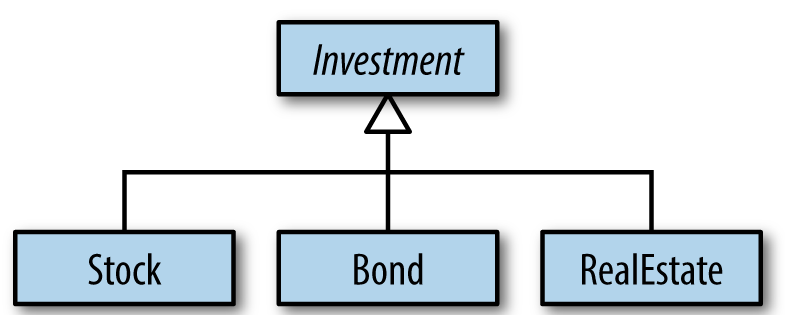
\includegraphics[width=10cm]{img/Snipaste_2021-05-26_14-20-43.png}

A factory function for such a hierarchy typically allocates an object on the heap and returns a pointer to it, with the caller being responsible for deleting the object when it’s no longer needed. That’s a perfect match for std::unique\_ptr, because the caller acquires responsibility for the resource returned by the factory (i.e., exclusive ownership of it), and the std::unique\_ptr automatically deletes what it points to when the std::unique\_ptr is destroyed. A factory function for the Investment hierarchy could be declared like this:

\begin{lstlisting}[language=C]
  template<typename... Ts>              // return std::unique_ptr
  std::unique_ptr<Investment>           // to an object created
  makeInvestment(Ts&&... params);       // from the given args

  auto delInvmt = [](Investment* pInvestment)       // custom
  {                                 // deleter
    makeLogEntry(pInvestment);      // (a lambda
    delete pInvestment;             // expression)
  };

template<typename... Ts>                          // revised
std::unique_ptr<Investment, decltype(delInvmt)>   // return type
makeInvestment(Ts&&... params) {
  std::unique_ptr<Investment, decltype(delInvmt)> // ptr to be
  pInv(nullptr, delInvmt);                      // returned

  if ( /* a Stock object should be created */ ) 
    pInv.reset(new Stock(std::forward<Ts>(params)...));
  else if ( /* a Bond object should be created */ ) 
    pInv.reset(new Bond(std::forward<Ts>(params)...));
  else if ( /* a RealEstate object should be created */ ) 
    pInv.reset(new RealEstate(std::forward<Ts>(params)...));

  return pInv;
}
\end{lstlisting}

\subsubsection{Use std::shared\_ptr for shared-ownership resource management.}
\begin{enumerate}
  \item std::shared\_ptrs are twice the size of a raw pointer, because they internally contain a raw pointer to the resource as well as a raw pointer to the resource’s reference count.2

  \item Memory for the reference count must be dynamically allocated. Conceptually, the reference count is associated with the object being pointed to, but pointed-to objects know nothing about this. They thus have no place to store a reference count. (A pleasant implication is that any object—even those of built-in types—may be managed by std::shared\_ptrs.) Item 21 explains that the cost of the dynamic allocation is avoided when the std::shared\_ptr is created by std::make\_shared, but there are situations where std::make\_shared can’t be used. Either way, the reference count is stored as dynamically allocated data.
  
  \item Increments and decrements of the reference count must be atomic, because there can be simultaneous readers and writers in different threads. For example, a std::shared\_ptr pointing to a resource in one thread could be executing its destructor (hence decrementing the reference count for the resource it points to), while, in a different thread, a std::shared\_ptr to the same object could be copied (and therefore incrementing the same reference count). Atomic operations are typically slower than non-atomic operations, so even though reference counts are usually only a word in size, you should assume that reading and writing them is comparatively costly.
\end{enumerate}

\begin{lstlisting}[language=C]
auto loggingDel = [](Widget *pw)        // custom deleter
  {                     // (as in Item 18)
    makeLogEntry(pw);
    delete pw;
  };

std::unique_ptr<                        // deleter type is
 Widget, decltype(loggingDel)          // part of ptr type
 > upw(new Widget, loggingDel);

std::shared_ptr<Widget>                 // deleter type is not
 spw(new Widget, loggingDel);          // part of ptr type
\end{lstlisting}
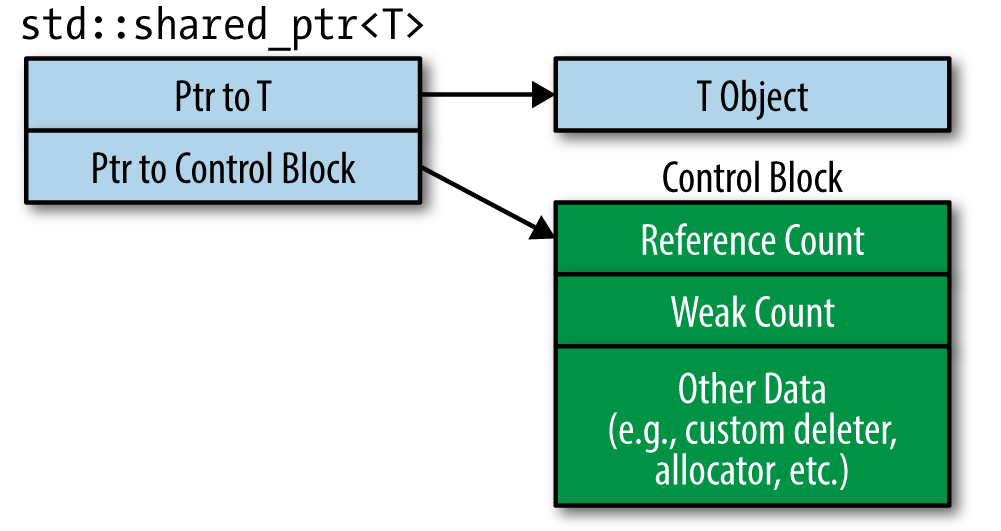
\includegraphics[width=10cm]{img/Snipaste_2021-05-26_14-26-09.png}

\subsubsection{Use std::weak\_ptr for std::shared\_ptr-like pointers that can dangle.}

As a final example of std::weak\_ptr’s utility, consider a data structure with objects A, B, and C in it, where A and C share ownership of B and therefore hold std::shared\_ptrs to it:

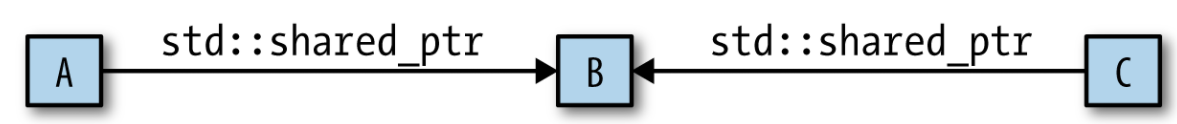
\includegraphics[width=10cm]{img/Snipaste_2021-05-26_14-32-03.png}
Suppose it’d be useful to also have a pointer from B back to A. What kind of pointer should this be?
\begin{enumerate}
  \item A raw pointer. With this approach, if A is destroyed, but C continues to point to B, B will contain a pointer to A that will dangle. B won’t be able to detect that, so B may inadvertently dereference the dangling pointer. That would yield undefined behavior.

  \item A std::shared\_ptr. In this design, A and B contain std::shared\_ptrs to each other. The resulting std::shared\_ptr cycle (A points to B and B points to A) will prevent both A and B from being destroyed. Even if A and B are unreachable from other program data structures (e.g., because C no longer points to B), each will have a reference count of one. If that happens, A and B will have been leaked, for all practical purposes: it will be impossible for the program to access them, yet their resources will never be reclaimed.
  
  \item A std::weak\_ptr. This avoids both problems above. If A is destroyed, B’s pointer back to it will dangle, but B will be able to detect that. Furthermore, though A and B will point to one another, B’s pointer won’t affect A’s reference count, hence can’t keep A from being destroyed when std::shared\_ptrs no longer point to it.
\end{enumerate}
Potential use cases for std::weak\_ptr include caching, observer lists, and the prevention of std::shared\_ptr cycles.
\subsection{Runtime Garbage Collector}
There are two main types of garbage collection algorithms, namely, tracing garbage collection algorithm and reference counting method. The three-color tagging method is one of the tracing garbage collection algorithms.

The core idea of tracing algorithm is to determine whether an object is reachable or not, because once the object is not reachable, it can be immediately reclaimed by GC. So how do we determine whether an object is reachable or not? The first step is to find all global variables and variables in the current function stack and mark them as reachable. In the second step, starting from the data already marked, further mark the variables they are accessible to, and so on, in the technical terminology called passing closures.

The Go language garbage collector has been evolving since day one, except for a few versions without major updates, almost every minor release improves the performance of garbage collection, and along with the performance improvement is the complexity of the garbage collector code, \href{https://draveness.me/golang/docs/part3-runtime/ch07-memory/golang-garbage-collector/}{this} section will analyze the evolution of the garbage collector starting from the Go language v1.0 version.

% \includegraphics[width=10cm]{img/v2-5fe8ea45e2518ca19cfeb31558160fb1_b.gif}
\begin{enumerate}
  \item v1.0 - a completely serial mark-and-clean process that requires pausing the entire program.
\item v1.1 - parallel execution of the mark and purge phases of garbage collection on a multicore host11.
\item v1.3 - runtime added support for accurate scanning of stack memory based on the assumption that only values of pointer types contain pointers, enabling truly accurate garbage collection12.
\item conversion of unsafe.Pointer types to values of integer types identified as illegitimate, potentially causing serious problems such as hanging pointers.
\item v1.5 - implemented a concurrent garbage collector based on a three-colored marker sweep13.
\item drastically reducing the garbage collection latency from several hundred ms to less than 10 ms.
\item calculating the appropriate time for garbage collection to start and accelerating the garbage collection process through concurrency.
\item v1.6 - implementation of a decentralized garbage collection coordinator.
\item explicitly based state machine enabling any Goroutine to trigger state migration for garbage collection.
\item using dense bitmaps instead of heap memory represented by idle chains to reduce CPU usage during the purge phase14.
\item v1.7 - reducing garbage collection time to less than 2ms by parallel stack shrinkage15.
\item v1.8 - reducing garbage collection time to within 0.5ms using a hybrid write barrier16.
\item v1.9 - completely removed the process of rescanning the stack for suspended procedures17.
\item v1.10 - updated the implementation of the garbage collection modulator (Pacer) to separate the soft and hard heap size targets18.
\item v1.12 - simplifying several phases of the garbage collector with a new marked termination algorithm19.
\item v1.13 - solving the problem of returning memory to the operating system for applications with excessive transient memory usage with a new Scavenger20.
\item v1.14 - optimizing the speed of memory allocation with a new page allocator21.
\end{enumerate}

\end{document}
